%&"../main"
\documentclass[../main]{subfiles}
\begin{document}

\chapter{公司介绍}%
\label{cha:公司介绍}

\section{公司简介}%
\label{sec:公司简介}

华为技术有限公司是一家生产销售通信设备的民营通信科技公司,于1987年正式注册成立,
总部位于中国广东省深圳市龙岗区坂田华为基地。华为是全球领先的信息与通信技术(ICT
)解决方案供应商,专注于ICT领域,坚持稳健经营、持续创新、开放合作,在电信运营商
、企业、终端和云计算等领域构筑了端到端的解决方案优势,为运营商客户、企业客户和消
费者提供有竞争力的ICT解决方案、产品和服务,并致力于实现未来信息社会、构建更美好
的全联接世界。2013年,华为首超全球第一大电信设备商爱立信,排名《财富》世界500强
第315位。

\begin{figure}[htbp]
	\centering
	
\includegraphics[width = 0.2\linewidth]{huawei.png}
	\caption{华为}
	\label{fig:华为}
\end{figure}

截至2016年底,华为有17多万名员工,华为的产品和解决方案已经应用于全球170多个国家
,服务全球运营商50强中的45家及全球1/3的人口,是一家不折不扣的跨国公司。

\newpage

\begin{figure}[htbp]
	\centering
	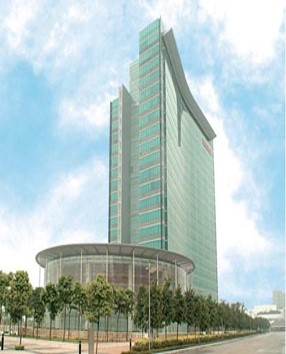
\includegraphics[width = 0.4\linewidth]{office.jpg}
	\caption{总部}
	\label{fig:总部}
\end{figure}

\section{服务理念}%
\label{sec:服务理念}

华为将继续秉承“以客户为中心”,基于客户需求,逐步建立在电信网络、全球服务和终端三
大业务领域的综合优势,为客户提供云、管、端产品和解决方案,帮助运营商改善收益
(ARPU)、提升带宽竞争力(Bandwidth) 和降低总拥有成本(Cost),实现商业成功。

\begin{figure}[htbp]
	\centering
	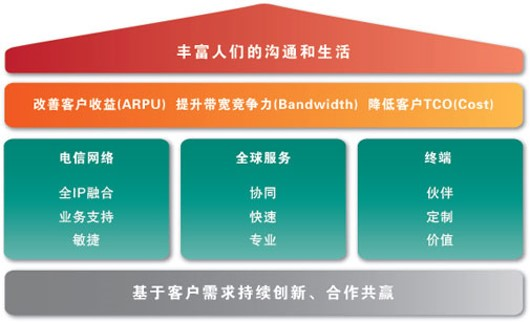
\includegraphics[width = 0.6\linewidth]{strategy.jpg}
	\caption{战略}
	\label{fig:战略}
\end{figure}

\end{document}

